After determining all of the cuts and corrections on 10$\%$ of the data, we applied these cuts and corrections unchanged to the entire data set (unblinding). The resulting vertex distribution is shown in Figure~\ref{fig:zVm_ub}.
\begin{figure}[htb]
  \centering
      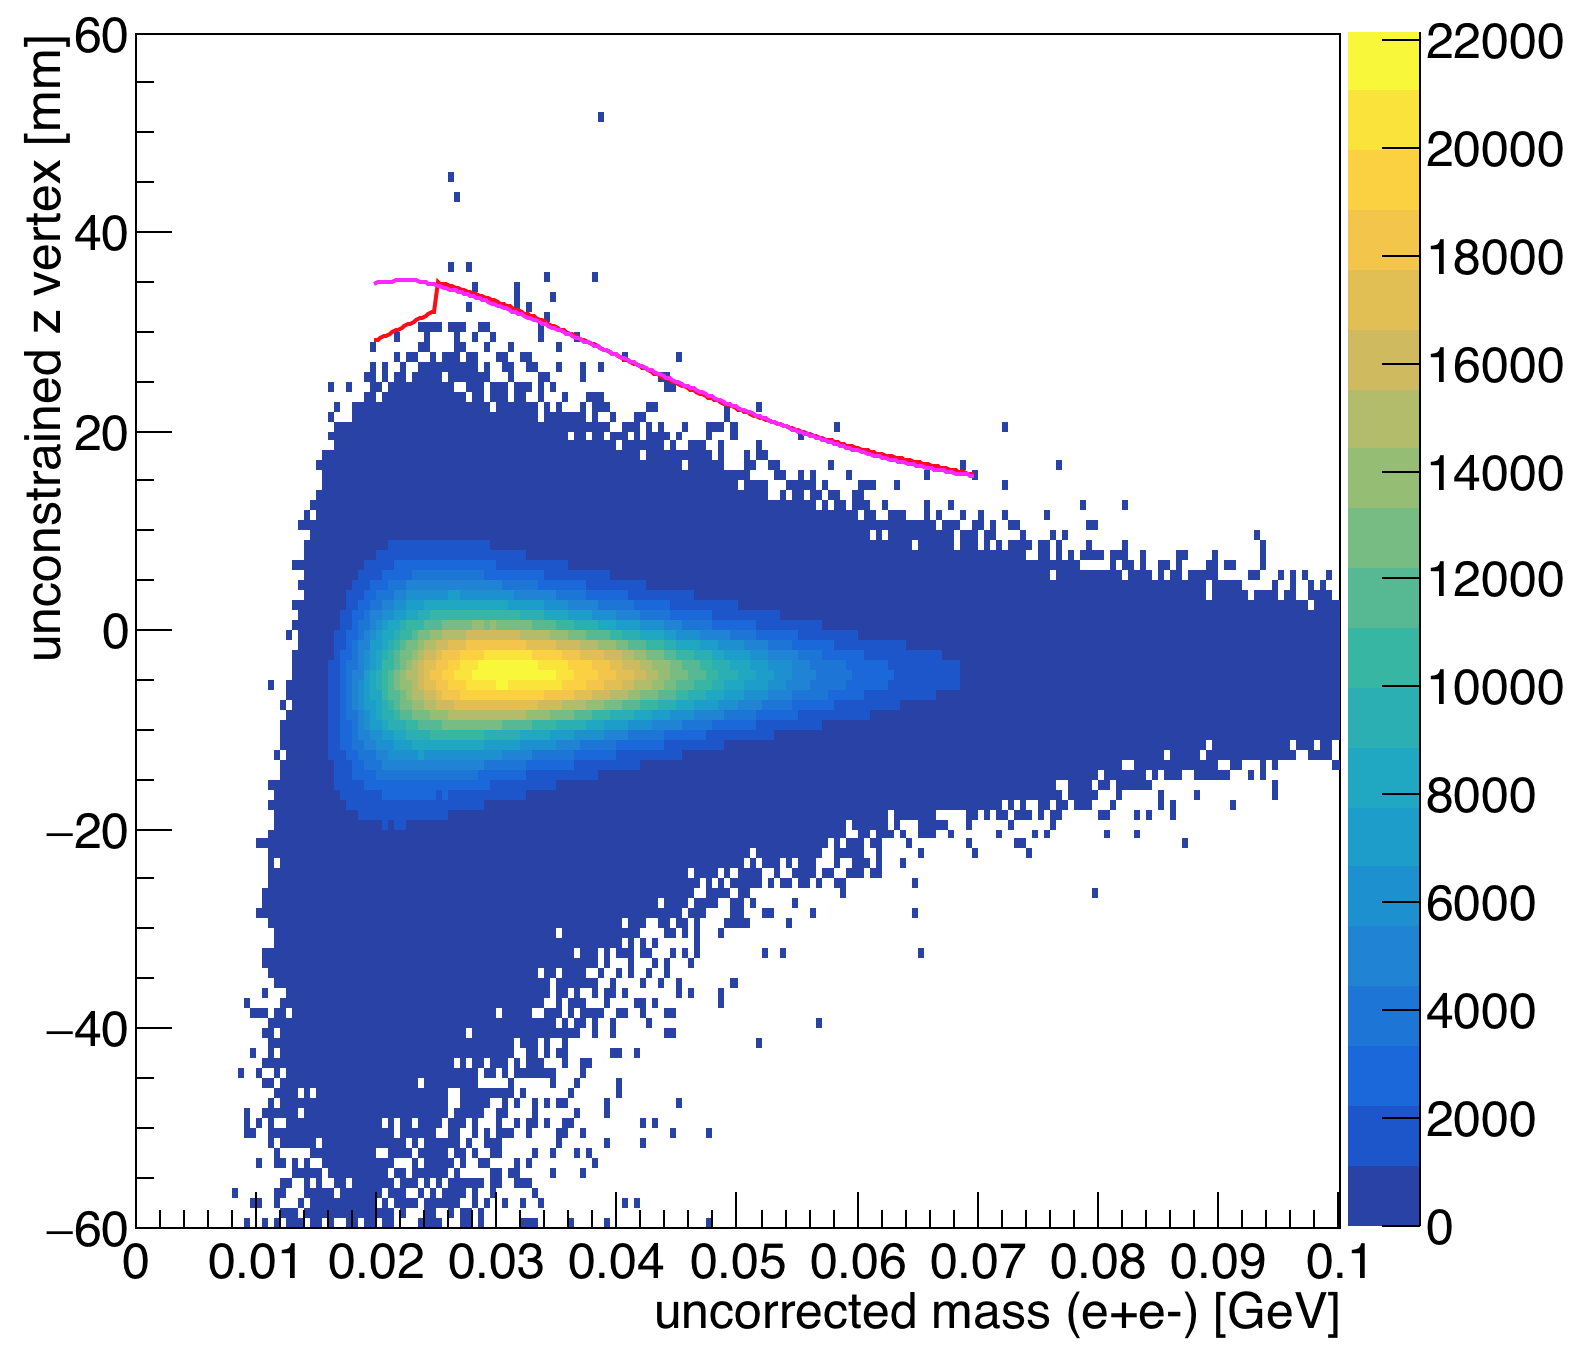
\includegraphics[width=0.75\textwidth]{pics/results/zVm_ub_L1L1.png}
  \caption[Vertex position vs mass for the 100$\%$ L1L1 data at 0.5~mm]{The unconstrained $z$ vertex position is shown as a function of the corrected mass of the $e^+e^-$ pair for 100$\%$ of the L1L1 data taken with the SVT at $\pm$0.5~mm from the beam. The $zCut$ as measured for this data is shown in red and corresponds to where there is less than 0.5 background events beyond. The projected $zCut$ from the 10$\%$ of the data is shown in magenta. The relevant mass range used to fit $zCut$ is from 0.02--0.08~GeV based on measured statistics.}
  \label{fig:zVm_ub}
\end{figure} 
The projected $zCut$ from the 10$\%$ sample agrees reasonably well with the $zCut$ measured from the full data vertex distribution. The $zCut$ is supposed to correspond to where one would measure less than 0.5 background events in the resolution-sized mass bin. As one can see from Figure~\ref{fig:zVm_ub}, there are significantly more events in the high $z$ region than expected. The distribution of these events as a function of mass is shown in Figure~\ref{fig:highz_mass}.
\begin{figure}[htb]
  \centering
      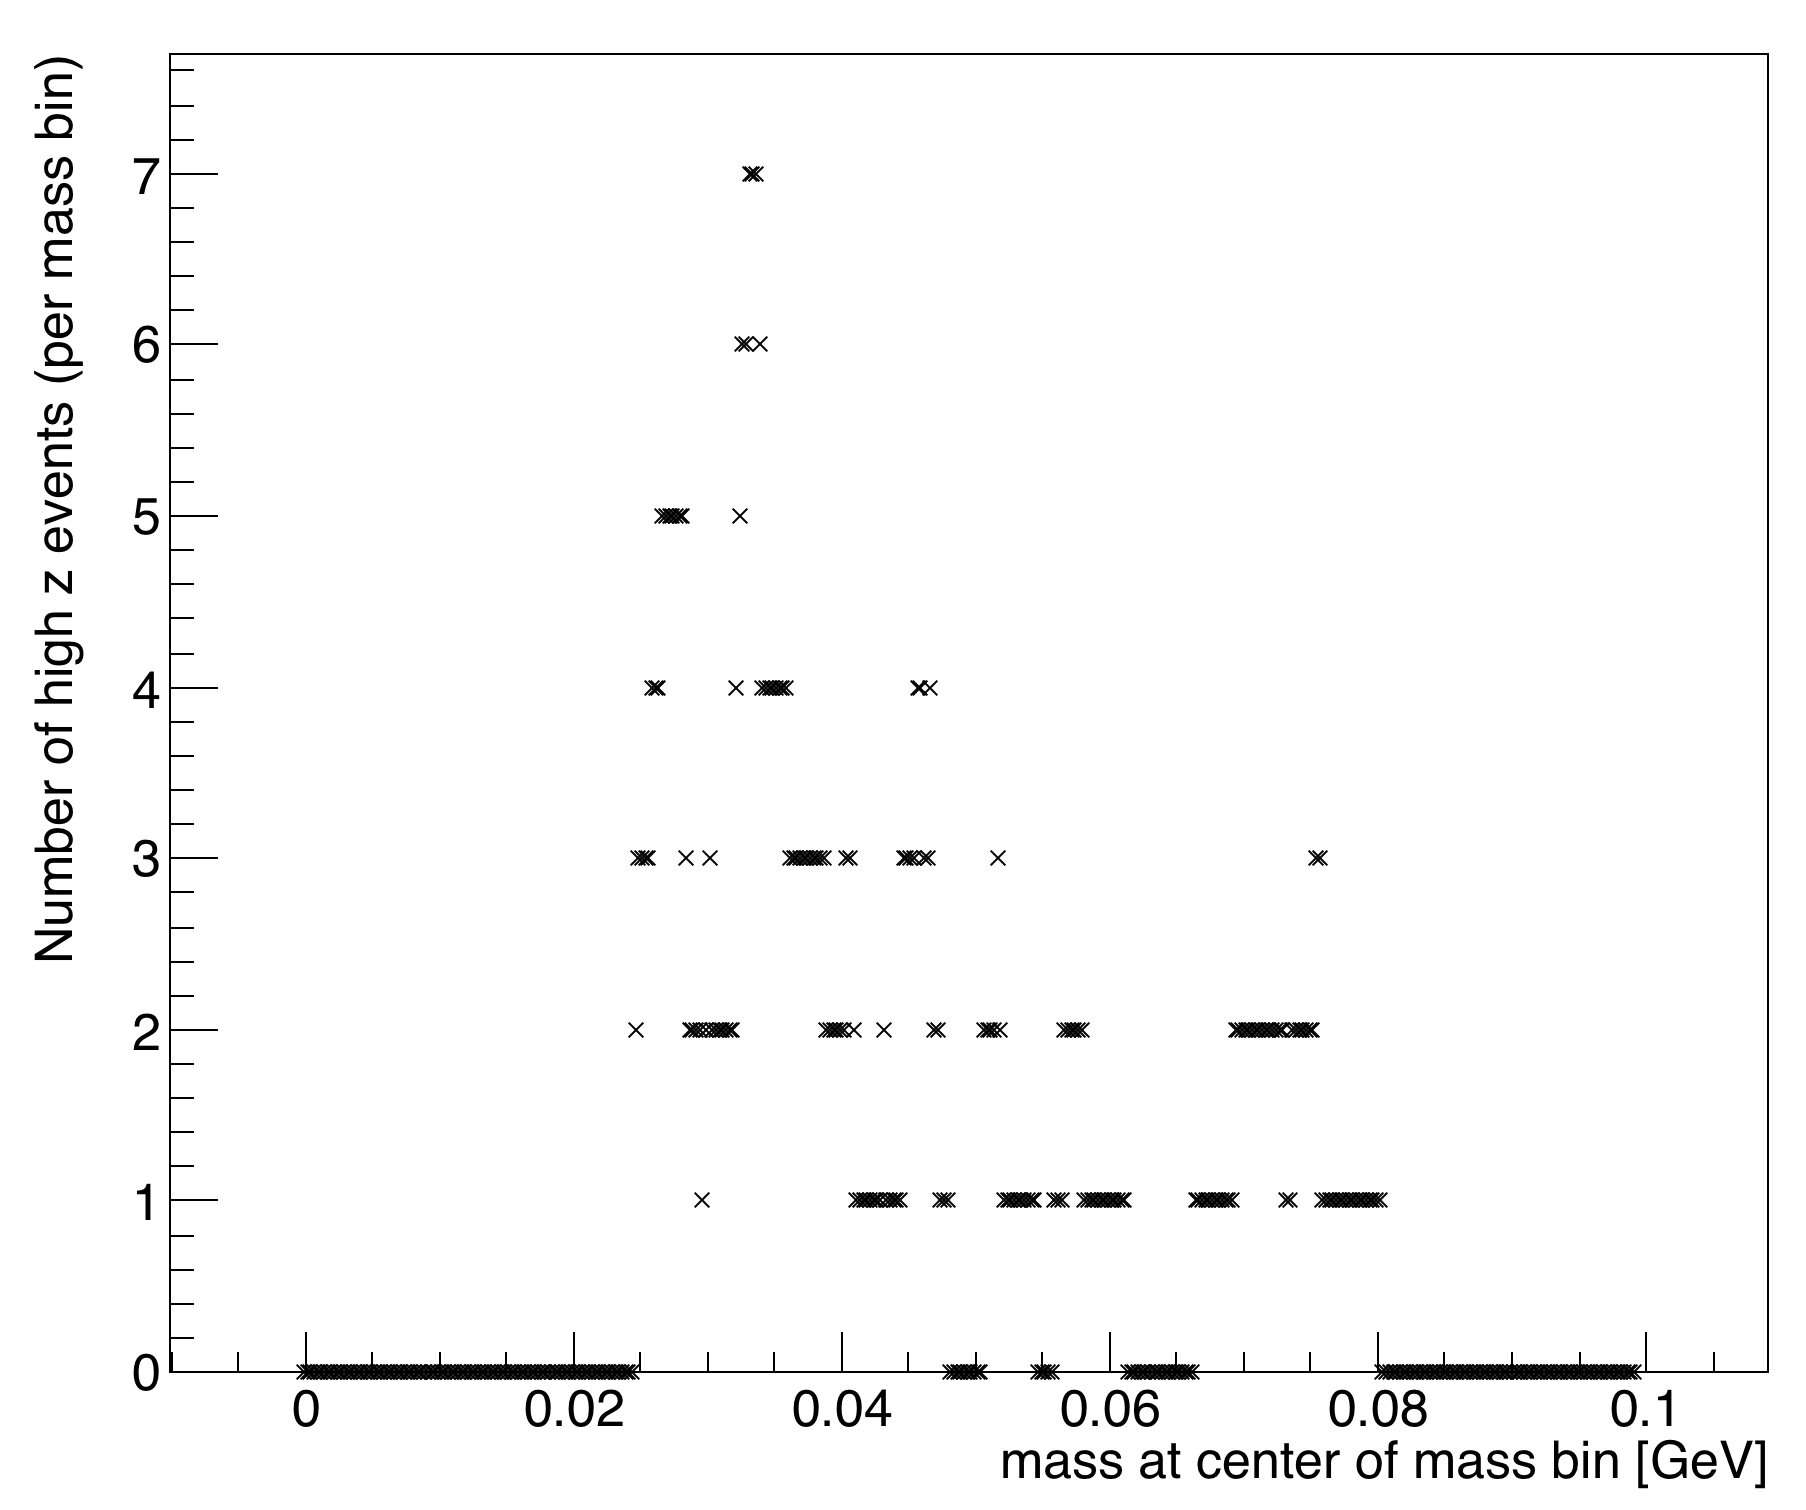
\includegraphics[width=0.75\textwidth]{pics/results/highz_v_mass.png}
  \caption[High $z$ events as a function of mass]{The high $z$ events from the full data set are shown as a function of their mass. Many of the events are plotted several times for the number of mass-resolution sized mass bins that they appear in. The highest number appear around 34~MeV, but the background is generally much higher than predicted across the full, measurable mass range.}
  \label{fig:highz_mass}
\end{figure} 
From choosing $zCut$ to correspond to 0.5 background events per mass bin, one would expect 6 high $z$ events across the range from 0.02 to 0.08~GeV. In reality, there are 24 events across this range. The distribution in mass peaks for the mass bin centered at 34~MeV but is generally much higher than predicted across the full, measurable range. The fit to the mass bin at 34~MeV containing the high number of excess background events is shown in Figure~\ref{fig:highz_34mev}.\\
\begin{figure}[htb]
  \centering
      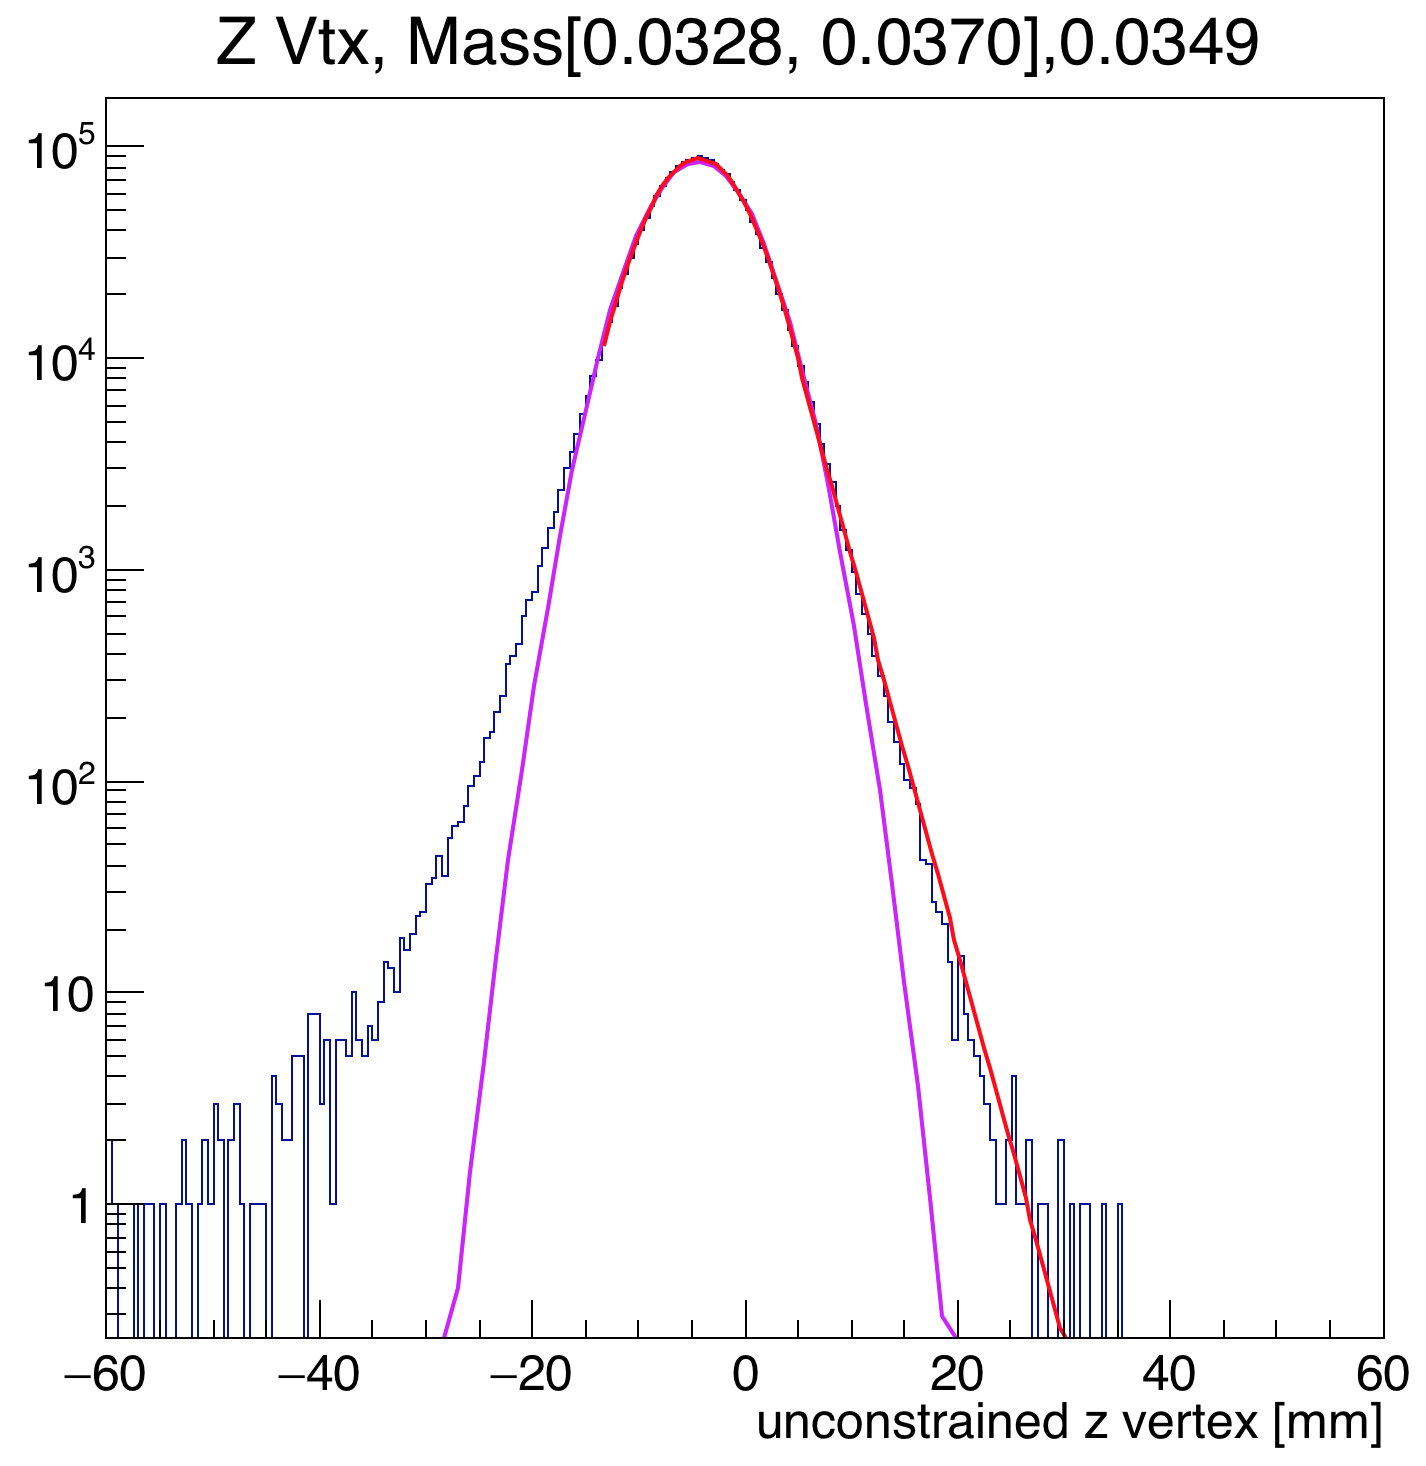
\includegraphics[width=0.65\textwidth]{pics/results/zvtx_34MeV.png}
  \caption[Vertex distribution for 34~MeV mass bin with high $z$ background]{The 34~MeV mass bin contains the highest number of background events beyond $zCut$.}
  \label{fig:highz_34mev}
\end{figure} 
\indent Because this is the full data that we are looking at and there could potentially be a heavy photon in the data set, we must be extremely careful in how we choose to characterize the excess background events. If we assume that the heavy photon will only appear in one mass bin, then one can very roughly estimate the measured background for a particular mass hypothesis by excluding events that fall in its mass range and measuring the average number of background events elsewhere. The average number of background events per mass bin, excluding those events in the mass hypothesis, is shown in Figure~\ref{fig:highz_newbg}.
\begin{figure}[htb]
  \centering
      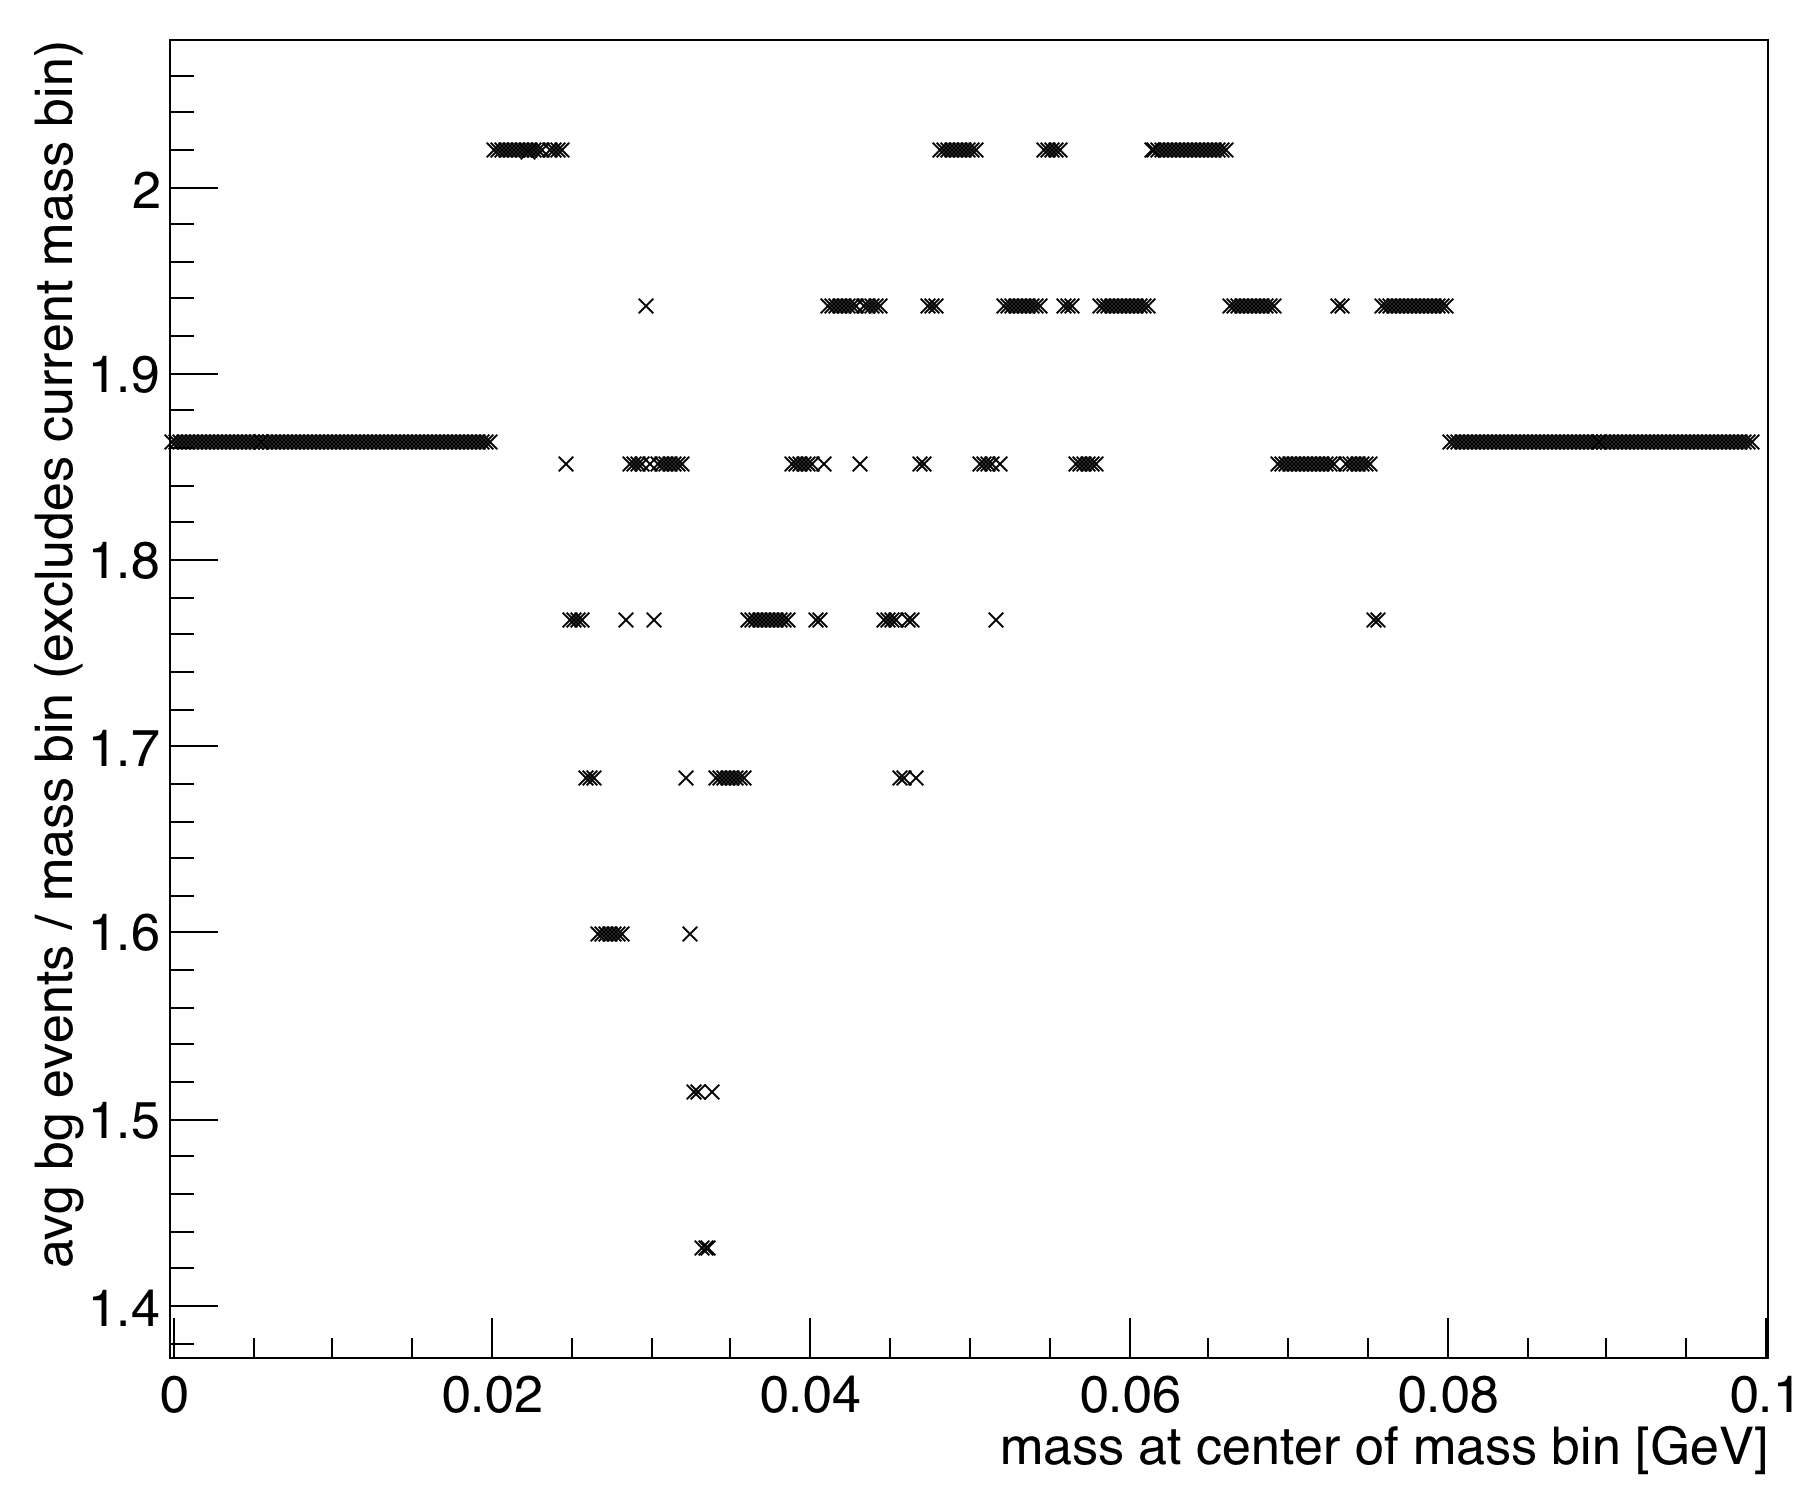
\includegraphics[width=0.75\textwidth]{pics/results/highz_avgBG.png}
  \caption[Re-characterization of the excess background]{The background events per mass bin are shown for each mass hypothesis by excluding the events that fall in that mass resolution-limited bin. This assumes that the heavy photon will fall in any one bin and results in a conservative background estimate for each bin.}
  \label{fig:highz_newbg}
\end{figure} 
The re-characterized background average ranged from 1.4 to just over 2 background events per mass bin. This is significantly higher than the expected 0.5 background events per mass bin. Ultimately, this distribution should be simulated and re-fit to be included in the $zCut$ calculation. For now, this is a sufficiently conservative estimate of the excess background and can be used to obtain the $p$-value associated with each mass hypothesis. \\
\indent The $p$-value is the probability in a background-only scenario to measure an apparent signal as significant as the data. Using the background as estimated from Figure~\ref{fig:highz_newbg}, we measure the following $p$-values in the fluctuations as shown in Figure~\ref{fig:highz_pval}.
\begin{figure}[htb]
  \centering
      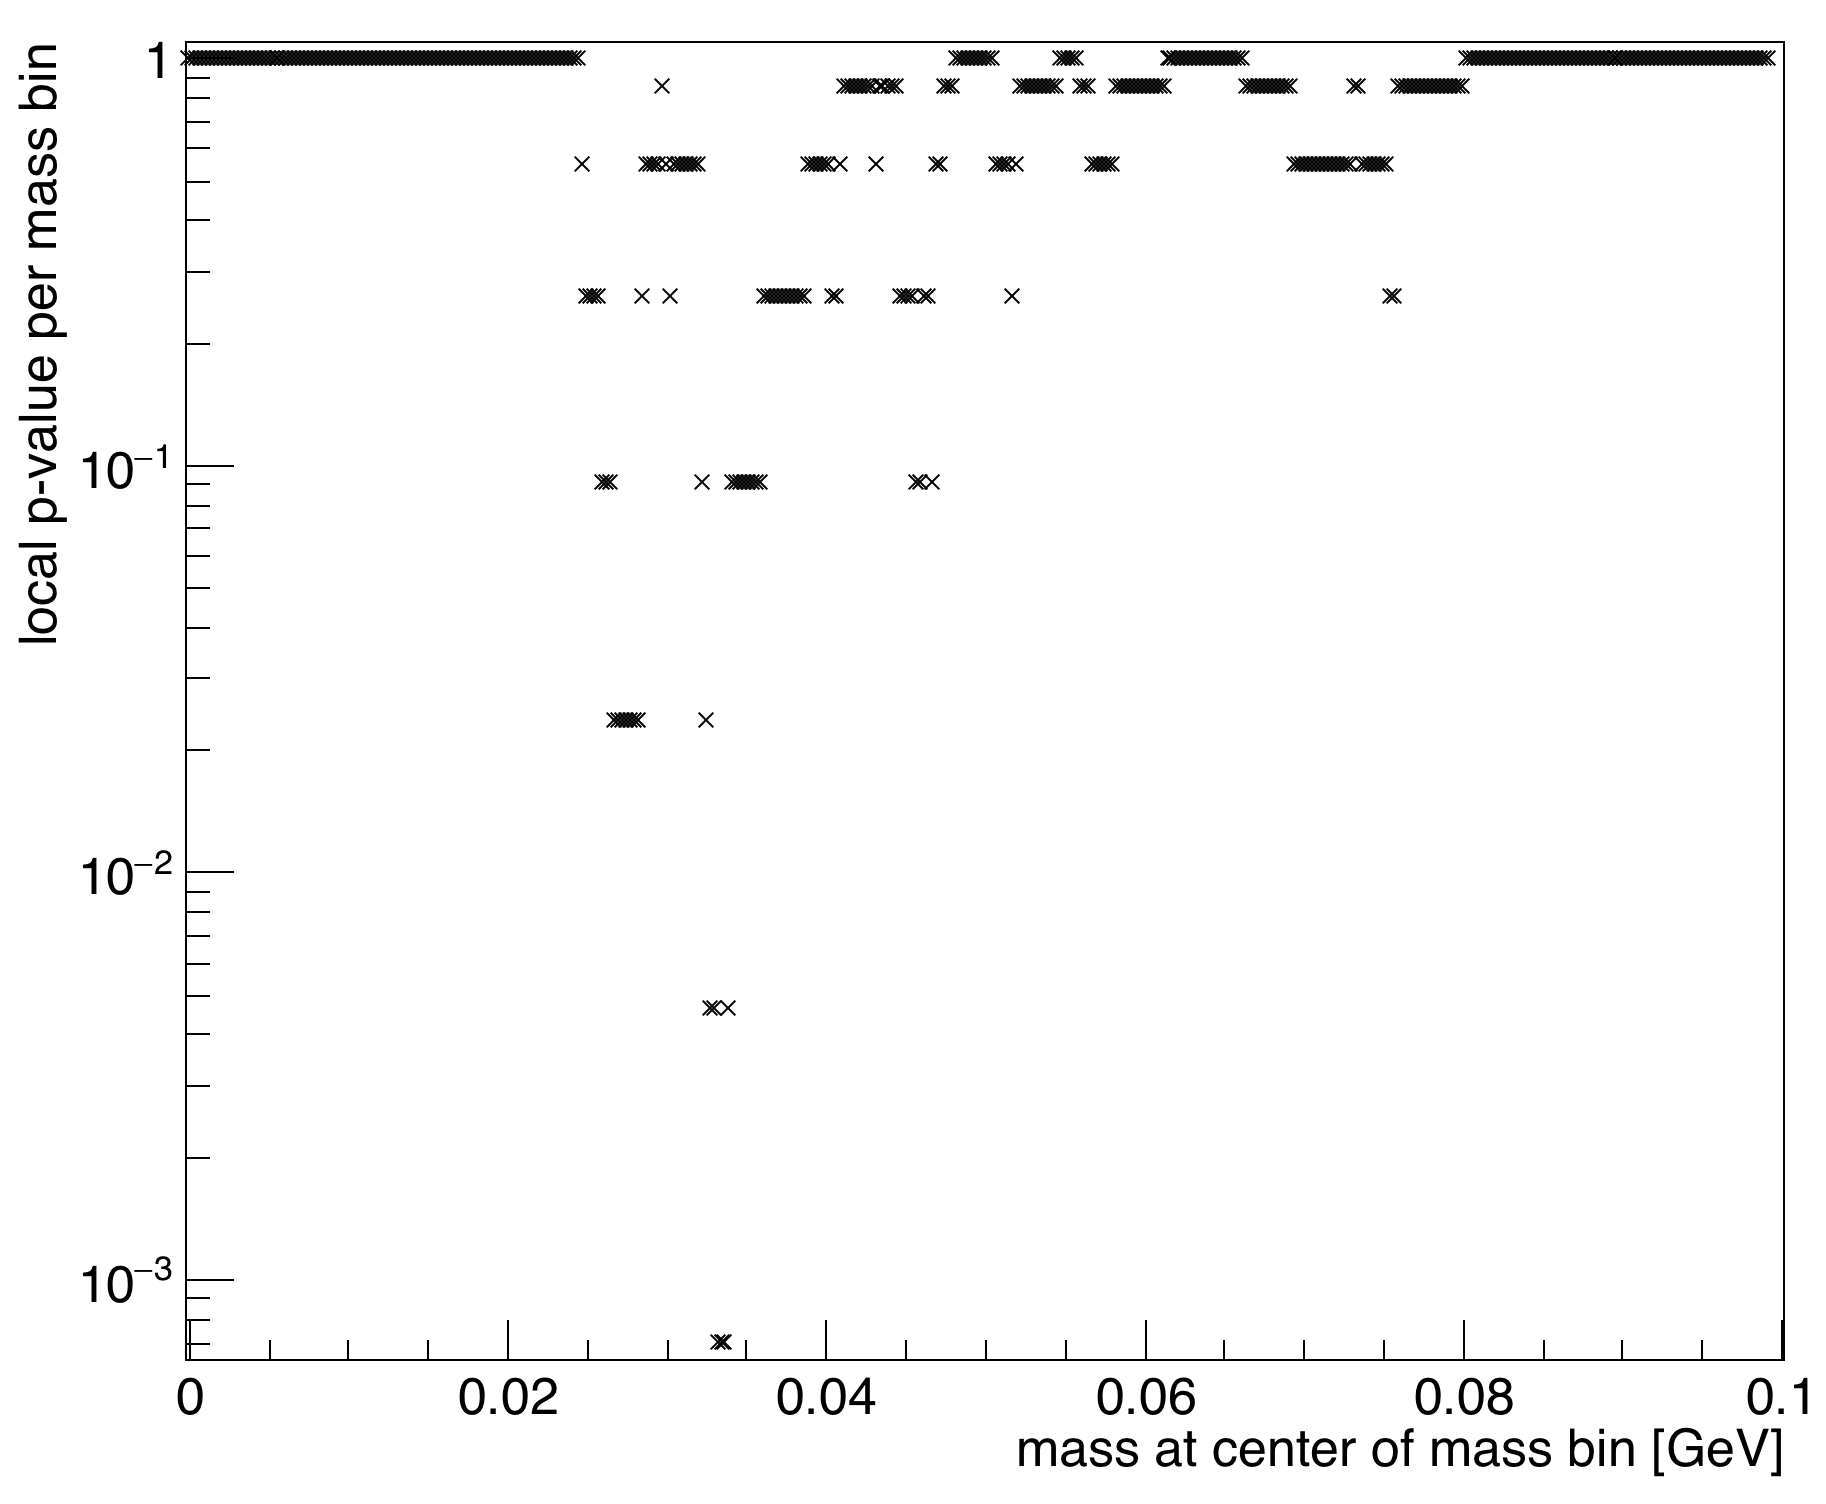
\includegraphics[width=0.75\textwidth]{pics/results/highz_pval.png}
  \caption[Local $p$--values for the L1L1 dataset]{The local $p$-values for each mass hypothesis using the data-characterized background estimate is shown. The $p$-value shows how well each hypothesis agrees with the background only model. The most significant $p$-value has a value of 0.00071 at approximately 34~MeV as this bin contains 7 high $z$ background events.}
  \label{fig:highz_pval}
\end{figure} 
The $p$-values shown in Figure~\ref{fig:highz_pval} are considered to be ``local" $p$-values as they only consider the significance of the events in a specific mass hypothesis and do not look at the significance of those events across the range of the full data. This is known as the Look Elsewhere Effect. In order to account for this effect, the local $p$-values need to be understood in terms of the global $p$-value in order to establish their significance for the full data set. The global $p$-value can be calculated by generating toy distributions using the same background model, and measuring the most significant local $p$-value for each data set. The local $p$-values for the toy distributions are ranked, and the quantile is calculated from this distribution that gives the mapping of the global $p$-value to the local $p$-values~\cite{gross_trial_2010}. The global $p$-value will always be less significant than the local $p$-value, by definition. By generating 10,000 toy vertex distributions from the background model in data and finding the most significant $p$-value in each simulation, one can obtain the mapping from local to global $p$-values. The mapping using toy distributions of the L1L1 0.5~mm data is shown in Figure~\ref{fig:pval_map}.

\begin{figure}[htb]
  \centering
      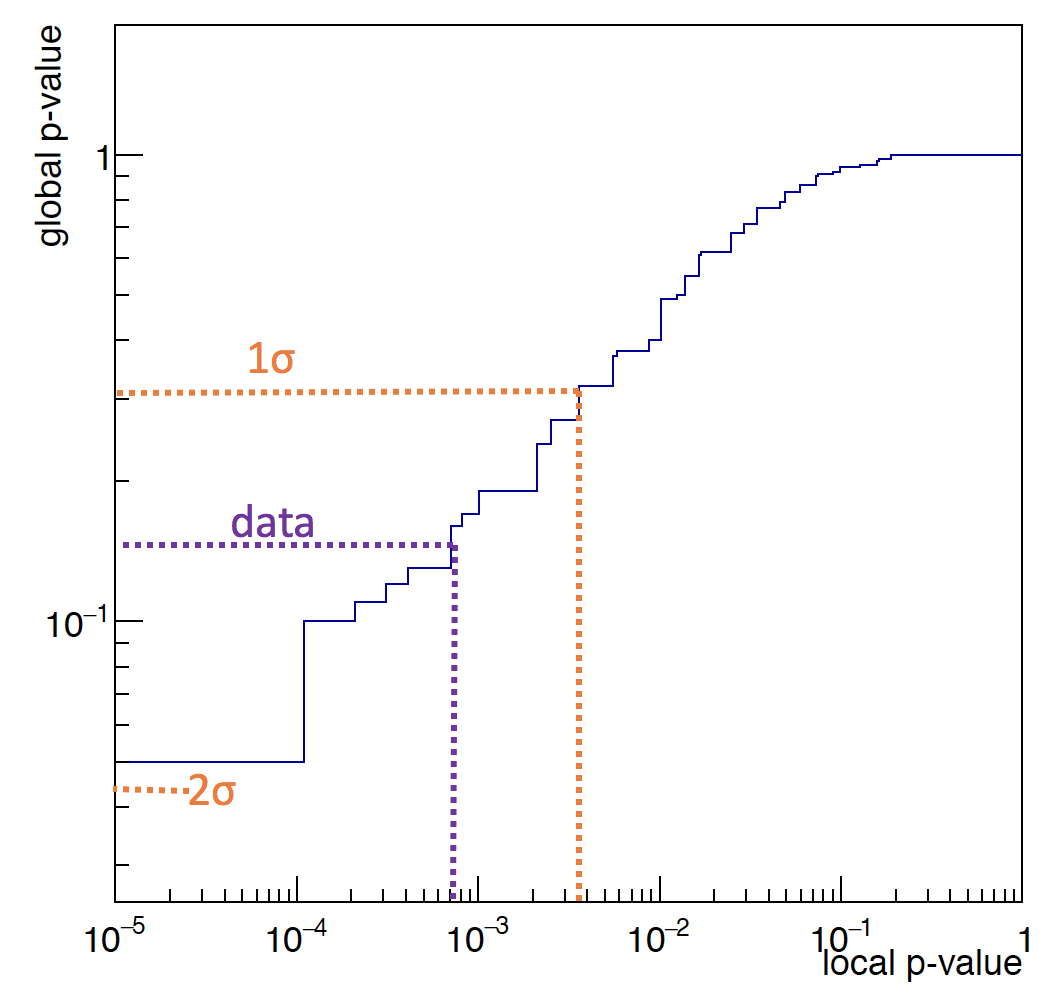
\includegraphics[width=0.75\textwidth]{pics/results/pvalMap.png}
  \caption[Mapping of local to global $p$--values]{The local to global $p$--value mapping is shown using 10,000 toy distributions modeled from the data. The orange dashed lines indicate the approximate locations of the global $p$-values as a significance in terms of a Gaussian fluctuation. The purple dashed line indicates the global $p$-value of the most significant fluctuation from the data (with local $p$-value of 0.00071) is 0.13. This translates to a Gaussian significance of 1.12$\sigma$.}
  \label{fig:pval_map}
\end{figure} 
The toy distributions are generated from sampling a two-dimensional parameterization of the $z$ vertex versus mass distribution from data. The function depends only on mass and $z$ vertex. From Equation~\eqref{eq:vtxFit}, all parameters that describe the distribution are mass dependent and can be obtained from the measured data. The two-dimensional generating function has an integral beyond $zCut$ yielding 0.5~background events per bin, as expected. In each generated toy model, the local $p$-value is obtained from recalculating the measured background in the surrounding bins (excluding that particular mass bin) and measuring the number of signal events in the given mass bin. In Figure~\ref{fig:pval_map}, the global $p$-values account for the significance of the fluctuations over the range of the data set. The most significant local $p$-value corresponds to a global $p$-value of 0.13 which can be expressed as a Gaussian significance of 1.12$\sigma$. Therefore, accounting for the presence of the unanticipated excess background, we did not observe any signal significance. \\
\indent Additionally, we can see the significance of the measured excess background events with respect to the background model by transforming the vertex slice fit into a cumulative distribution function. We can see the deviation of the measured $z$ vertex position with respect to the model as the quantile of $1-e^{(z_{cut}-z)/l}$. For high $z$ events that agree well with the background hypothesis, the quantile is closer to 0. Those events that deviate with respect to the background hypothesis will be closer to 1. These values are shown in Figure~\ref{fig:highz_quantile}.
\begin{figure}[htb]
  \centering
      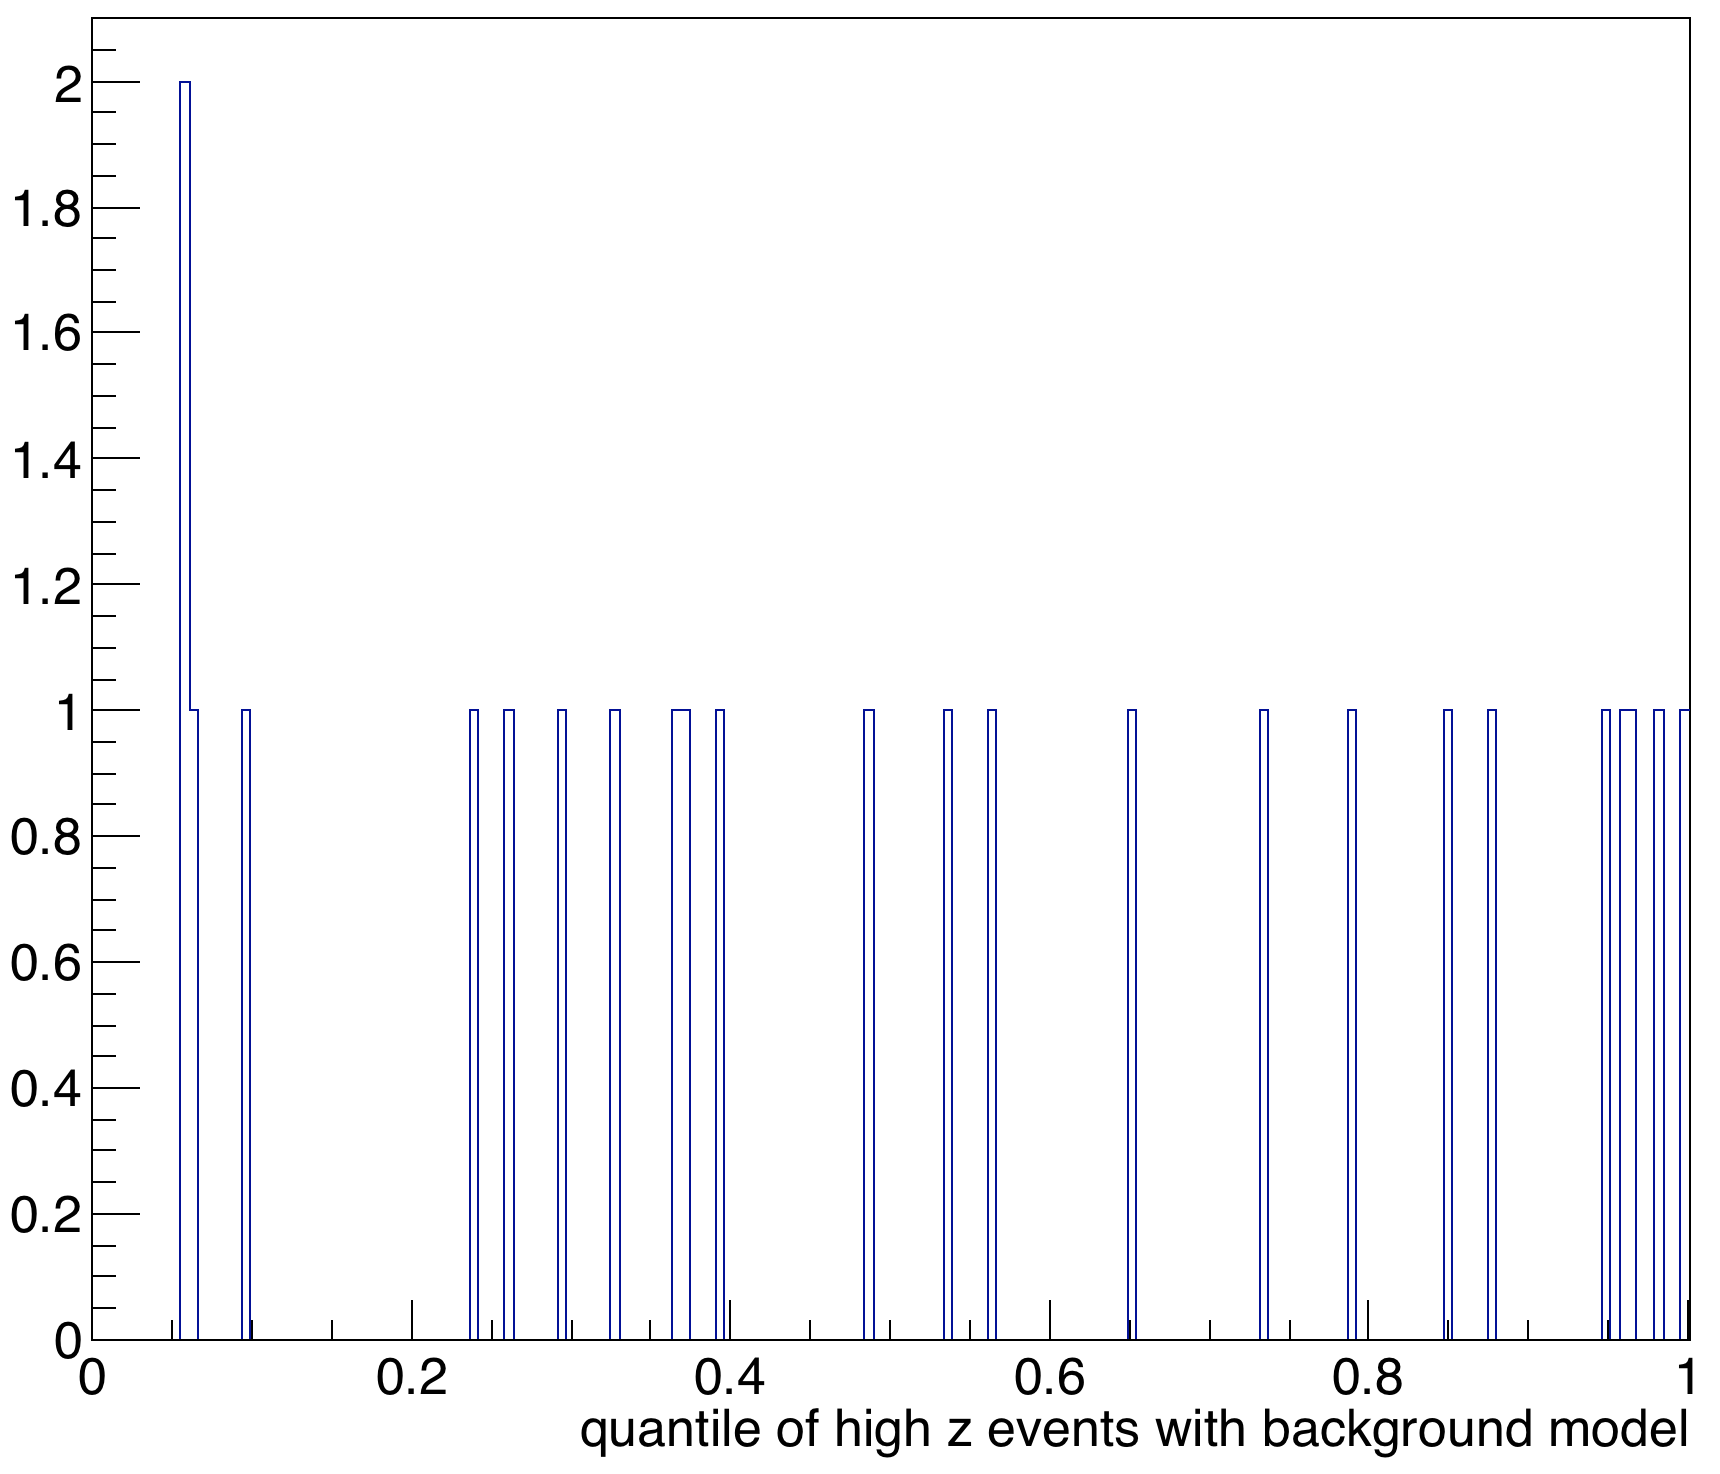
\includegraphics[width=0.75\textwidth]{pics/results/highz_quantiles.png}
  \caption[Deviation of the measured high $z$ event from the background $zCut$]{The deviation of the measured high $z$ event from the background is defined by the quantile of the cumulative distribution function $1-e^{(z_{cut}-z)/l}$. Events that are consistent with the hypothesis are close to 0 while those events that differ greatly from the hypothesis are closer to 1.}
  \label{fig:highz_quantile}
\end{figure} 
There are five events that are clustered close to 1 having a significant deviation with respect to the background $zCut$ hypothesis. The remainder of the events are spread fairly evenly across all mass hypotheses. These events with the greatest difference will lie farthest from the $zCut$ and are mostly centered around the 34~MeV mass bin which also contains the largest signal fluctuation. In order to obtain the correct amount of high $z$ events across the distribution, one would need to move the $zCut$ downstream by 4~mm. This still would have one mass bin containing 3~events. By moving the $zCut$ 5~mm downstream, no mass resolution-sized bin would contain more than 2~events. 

\subsection{Discussion of the L1L1 data with the SVT at $\pm$1.5~mm}
The 1.5~mm L1L1 data set has many fewer events than the 0.5~mm data but also has significantly fewer background events. The full vertex distribution is shown in Figure~\ref{fig:zVm1p5_ub}.
\begin{figure}[htb]
  \centering
      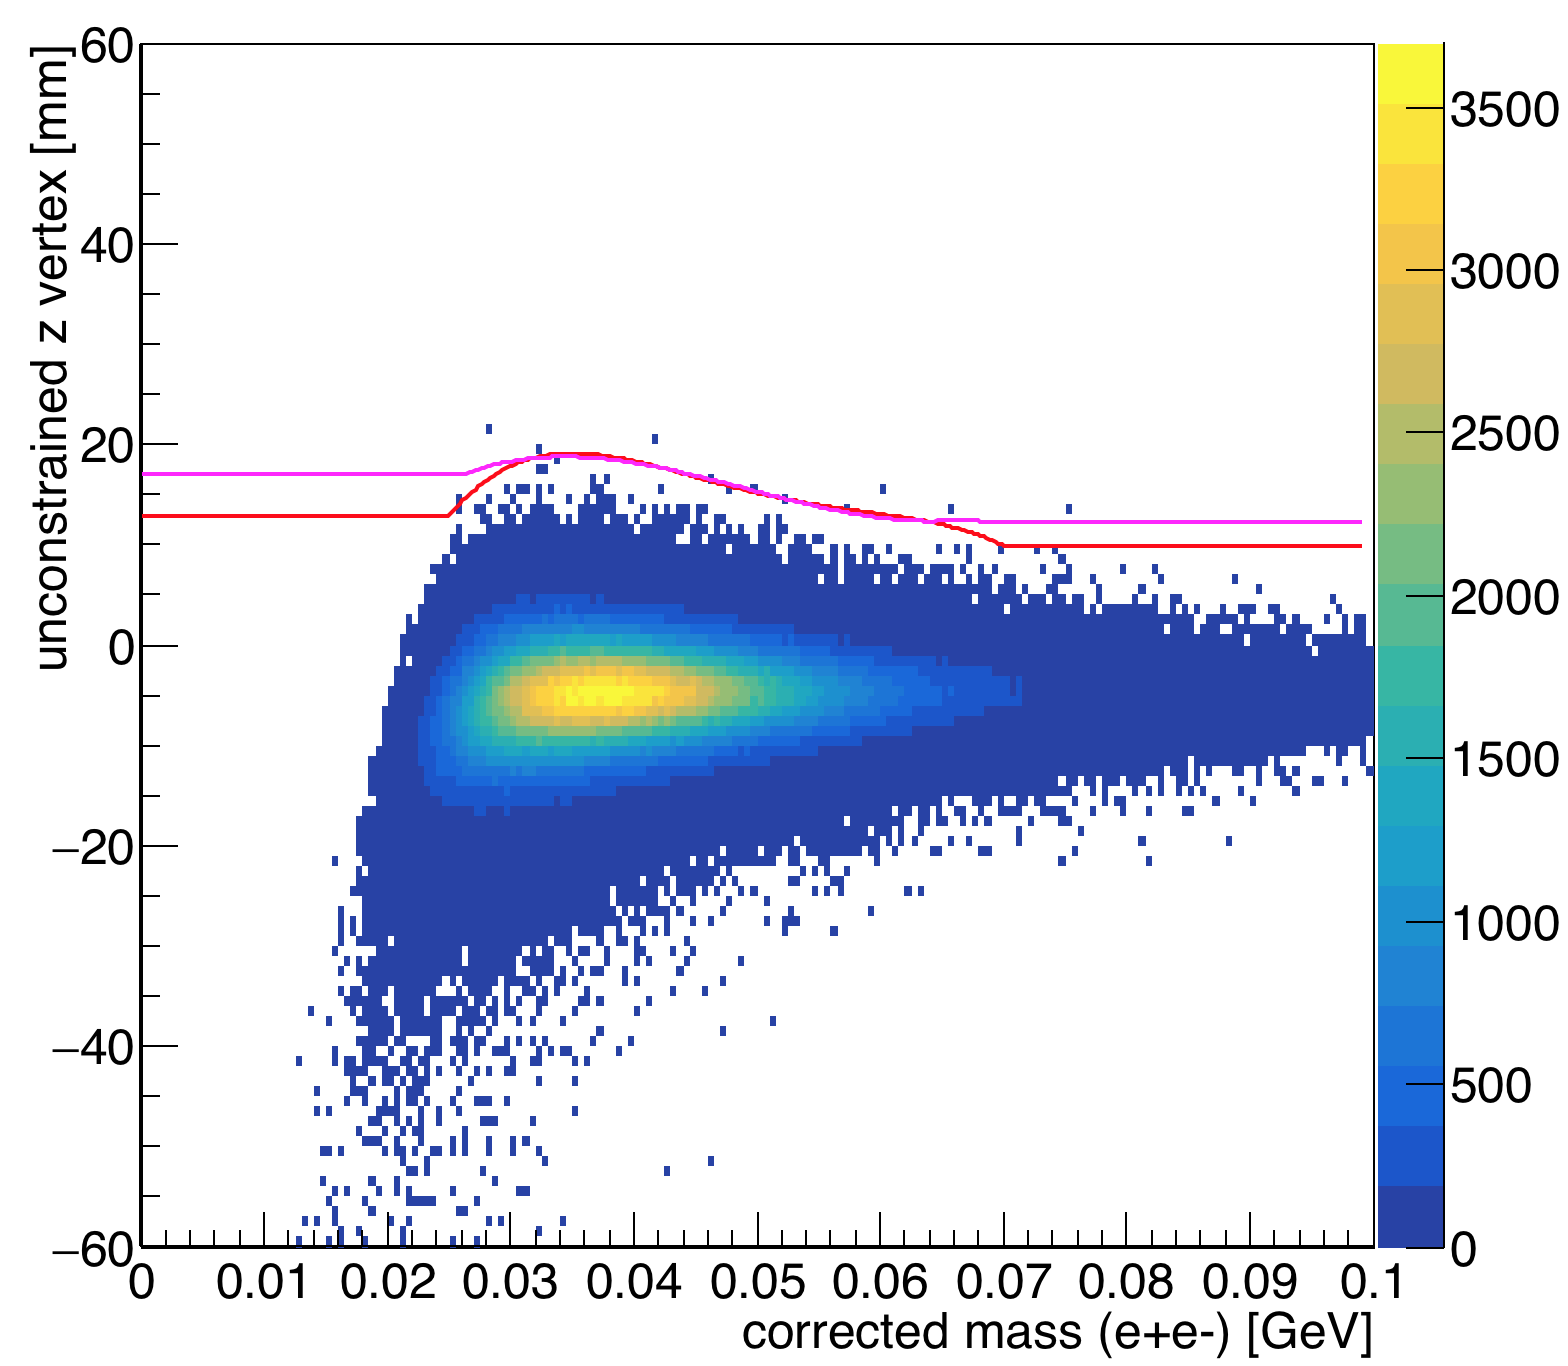
\includegraphics[width=0.75\textwidth]{pics/results/zVm_1p5mm.png}
  \caption[Vertex position vs mass for the 100$\%$ L1L1 data at 1.5~mm]{The unconstrained $z$ vertex position is shown as a function of the corrected mass of the $e^+e^-$ pair in events with the SVT at $\pm1.5$~mm from the beam. The $zCut$ as measured for this data is shown in red and corresponds to where there is less than 0.5 background events beyond. The projected $zCut$ from the 10$\%$ of the data is shown in magenta. The relevant mass range used to fit $zCut$ is from 0.024--0.07~GeV based on measured statistics.}
  \label{fig:zVm1p5_ub}
\end{figure} 
If we consider the high $z$ background in the 1.5~mm data set, we see that the average number of background events throughout the mass range is around 0.8 events per resolution-sized mass bin. Additionally, there are at most 2 events in a single one of the resolution-sized bins. If we exclude the three events that lie on the $zCut$ (either by agreement with the background model or moving the $zCut$ by 1~mm farther downstream), then we obtain an average of 0.51 events per resolution-sized mass bin. This seems to indicate that most of the high $z$ events in the 0.5~mm data set come from scatters in the dead region of Layer 1, probably due to the high rates and close proximity to the beam.

\section{Reach}
As mentioned previously, the reconstruction algorithm does not accurately propagate track parameters back to the displaced $z$ vertex position. The track parameters used to calculate the mass were those found at the pre-determined interaction point and not at the found vertex position. The $x$--component of the momentum was the track parameter that was most significantly affected. For now, if we assume that by fixing the vertexing algorithm we would have resolution good enough to remove the excess high $z$ background events and not lose statistics in the core of the distribution, then we can estimate the potential reach. The ``reach" is our ability to exclude phase space in mass and $\epsilon^2$. Using Equation~\eqref{eq:signal}, the 90$\%$ confidence limit is attained where we can expect at least 2.303 signal events. Assuming the same number of statistics in the core of the distribution but less background in the high $z$ region, the upper limit signal measurable from the L1L1 data sets is shown in Figure~\ref{fig:L1L1_reach}.
\begin{figure}[htb]
  \centering
      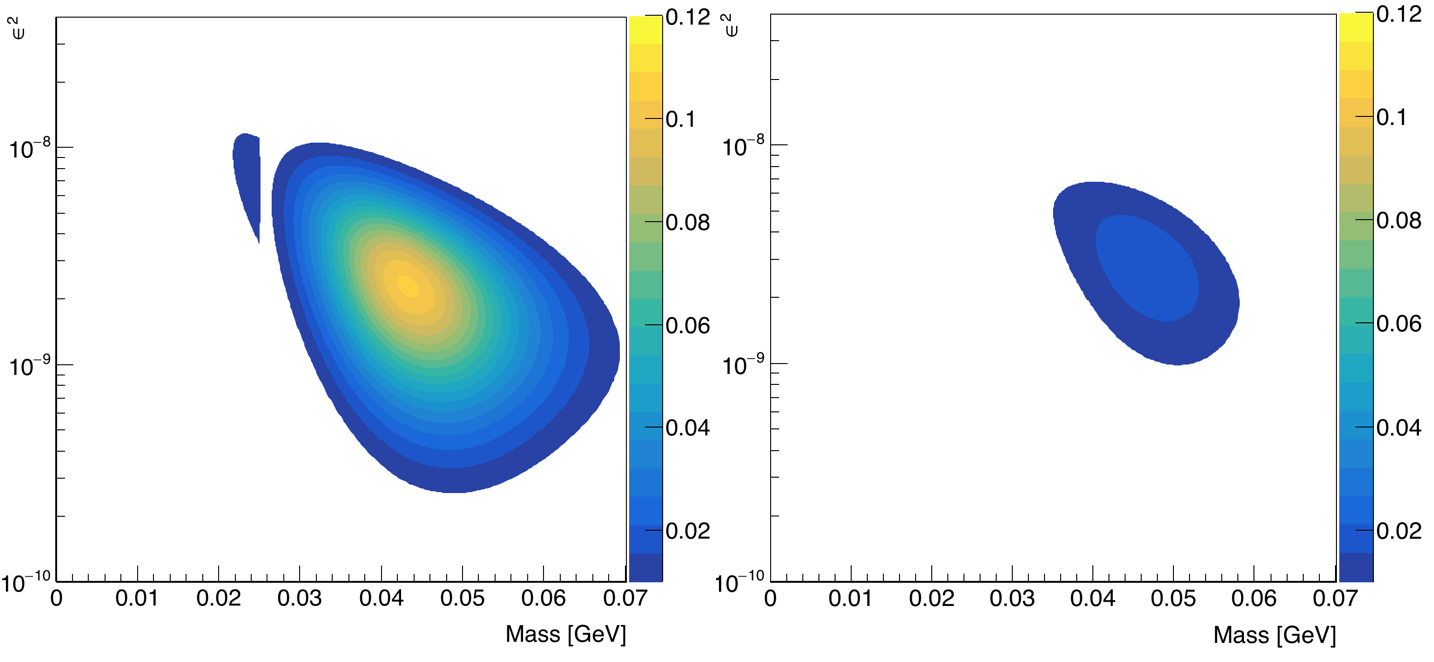
\includegraphics[width=0.9\textwidth]{pics/results/reach_sets.png}
  \caption[Expected signal yield for the individual L1L1 data sets]{The expected signal yield as calculated from Equation~\eqref{eq:signal} is shown for the 0.5~mm L1L1 data on the left and the 1.5~mm L1L1 data on the right. The highest signal expected from the 0.5~mm data is 0.109 events.}
  \label{fig:L1L1_reach}
\end{figure} 
Figure~\ref{fig:L1L1_reach} shows the upper limit signal yield for the 0.5~mm and 1.5~mm L1L1 data sets separately. Other data sets with different layer combinations are shown in the Appendix~\ref{appendix:reach}. In the 0.5~mm data, the L1L2 data is contaminated with high $z$ events that force the $zCut$ to be too large to attain any reach. The L1L2 data with the SVT at $\pm$1.5~mm has very little contamination of high $z$ background events but has too little statistics to contribute to the reach. The L2L2 data set from the 0.5~mm data has a large background in the high $z$ region and very low overall statistics that make fitting a $zCut$ impossible. The L2L2 data set from the 1.5~mm data has a large $zCut$ and low statistics that do not contribute to the overall signal yield. The combined limits from the 0.5~mm and 1.5~mm L1L1 data sets is shown in Figure~\ref{fig:comb_reach} where the maximum attainable signal is 0.121 events. 
\begin{figure}[htb]
  \centering
      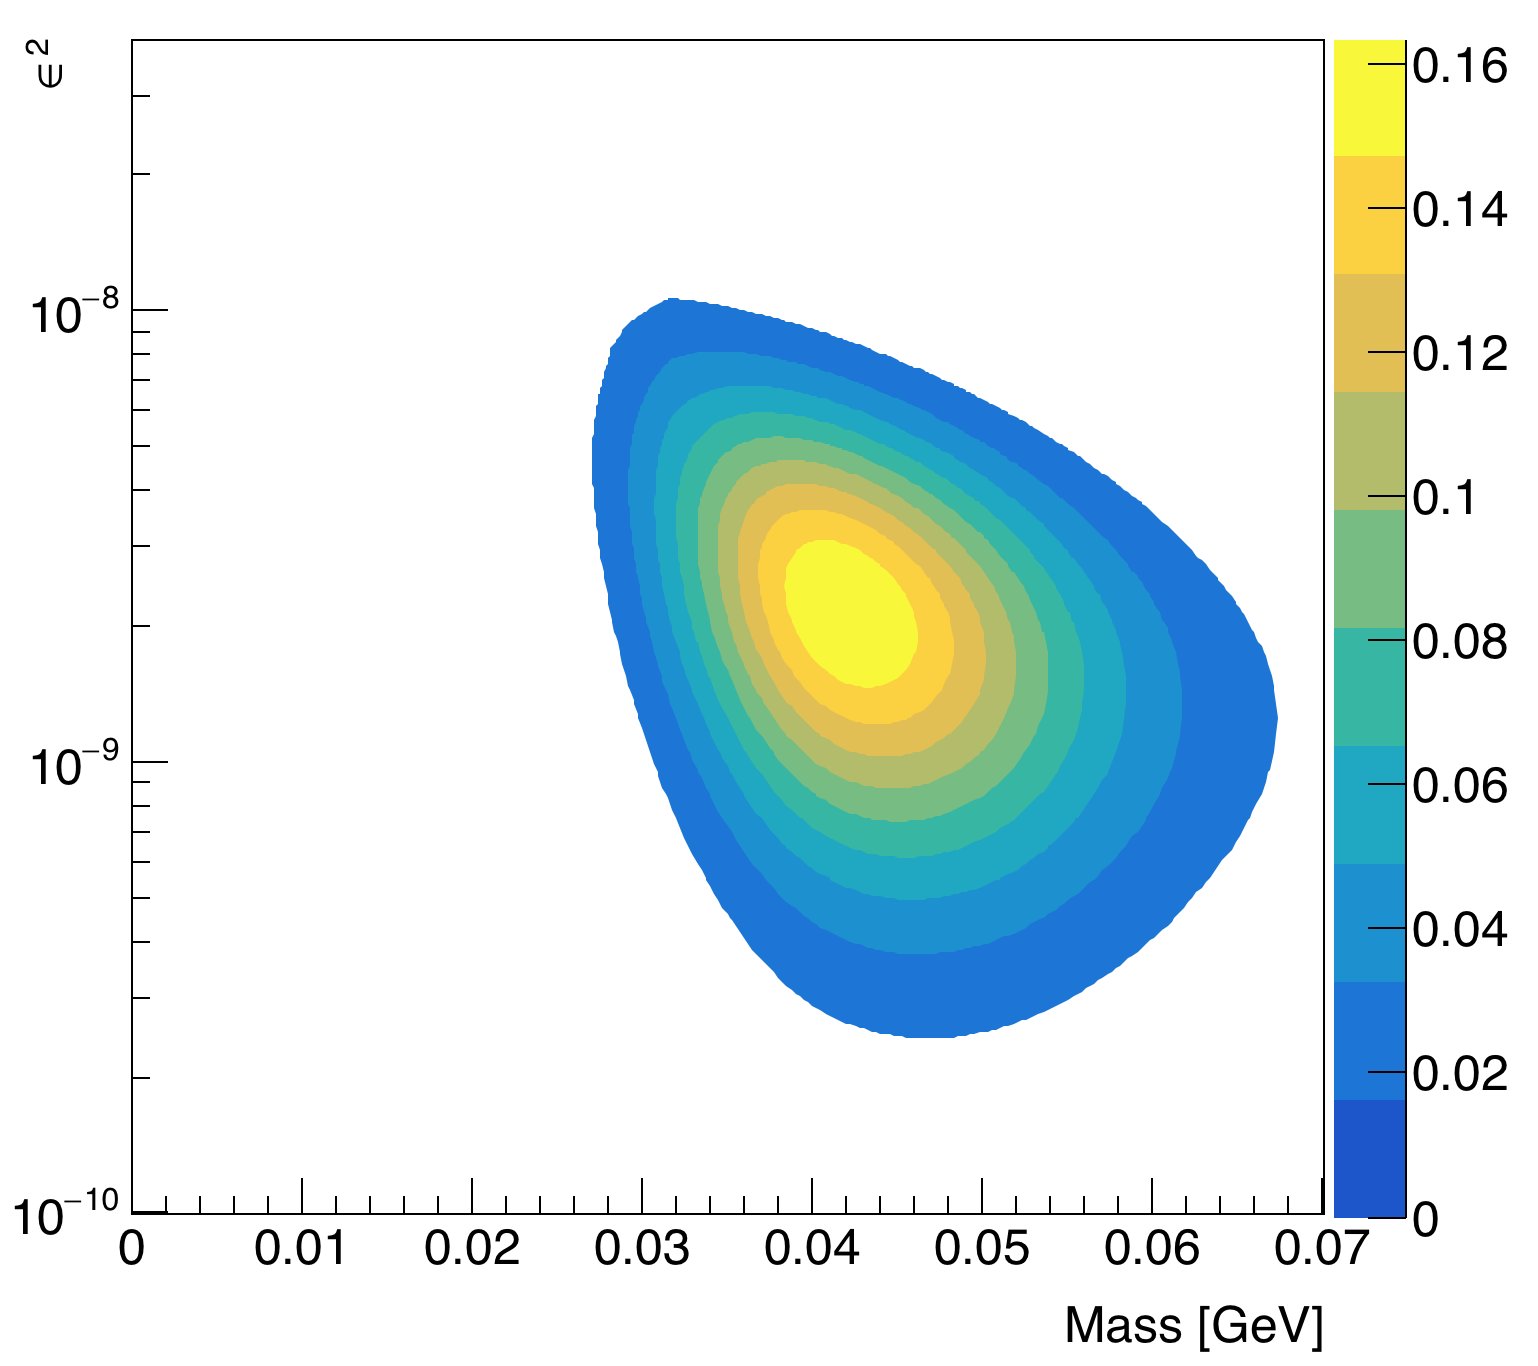
\includegraphics[width=0.55\textwidth]{pics/results/combinedReach.png}
  \caption[Combined reach from all data for the 2015 engineering run]{The combined reach for the 0.5~mm and 1.5~mm data is shown with the maximum signal expected to the be 0.121 events.}
  \label{fig:comb_reach}
\end{figure} 
As the maximum signal is significantly less than that required for the 90$\%$ confidence level, no regions of mass -- $\epsilon^2$ phase space were excluded by the 2015 engineering run. The $zCut$ was projected from the 10$\%$ data to the 100$\%$ data using the following relation obtained from the fits to the vertex distribution (from Equation~\eqref{eq:vtxFit}):
\begin{equation}
\label{eq:zProjected}
z_{2} = z_{1} - l\ln(A_1/A_2)
\end{equation}
where the subscript 1 indicates the known (10$\%$) data and the subscript 2 indicates the projected (100$\%$) data. The ratio of the amplitudes $A_1/A_2$ of the core distribution is used to estimate the change in statistics, $z$ is the $zCut$, and $l$ is the parameter to describe the length of the exponential tail that varies as a function of mass. This relationship can be used to project the $zCut$ for future run times from this data. 

%By projecting the $zCut$ and the statistics of the 0.5~mm data set, no reach would have been attainable until close to 12~weeks of continuous running. Additionally, the reach that can be obtained for one year of running still covers much less territory in coupling and mass than that expected from the proposal as shown in Figure~\ref{fig:reach_1yr}.
%
%\begin{figure}[htb]
%  \centering
%      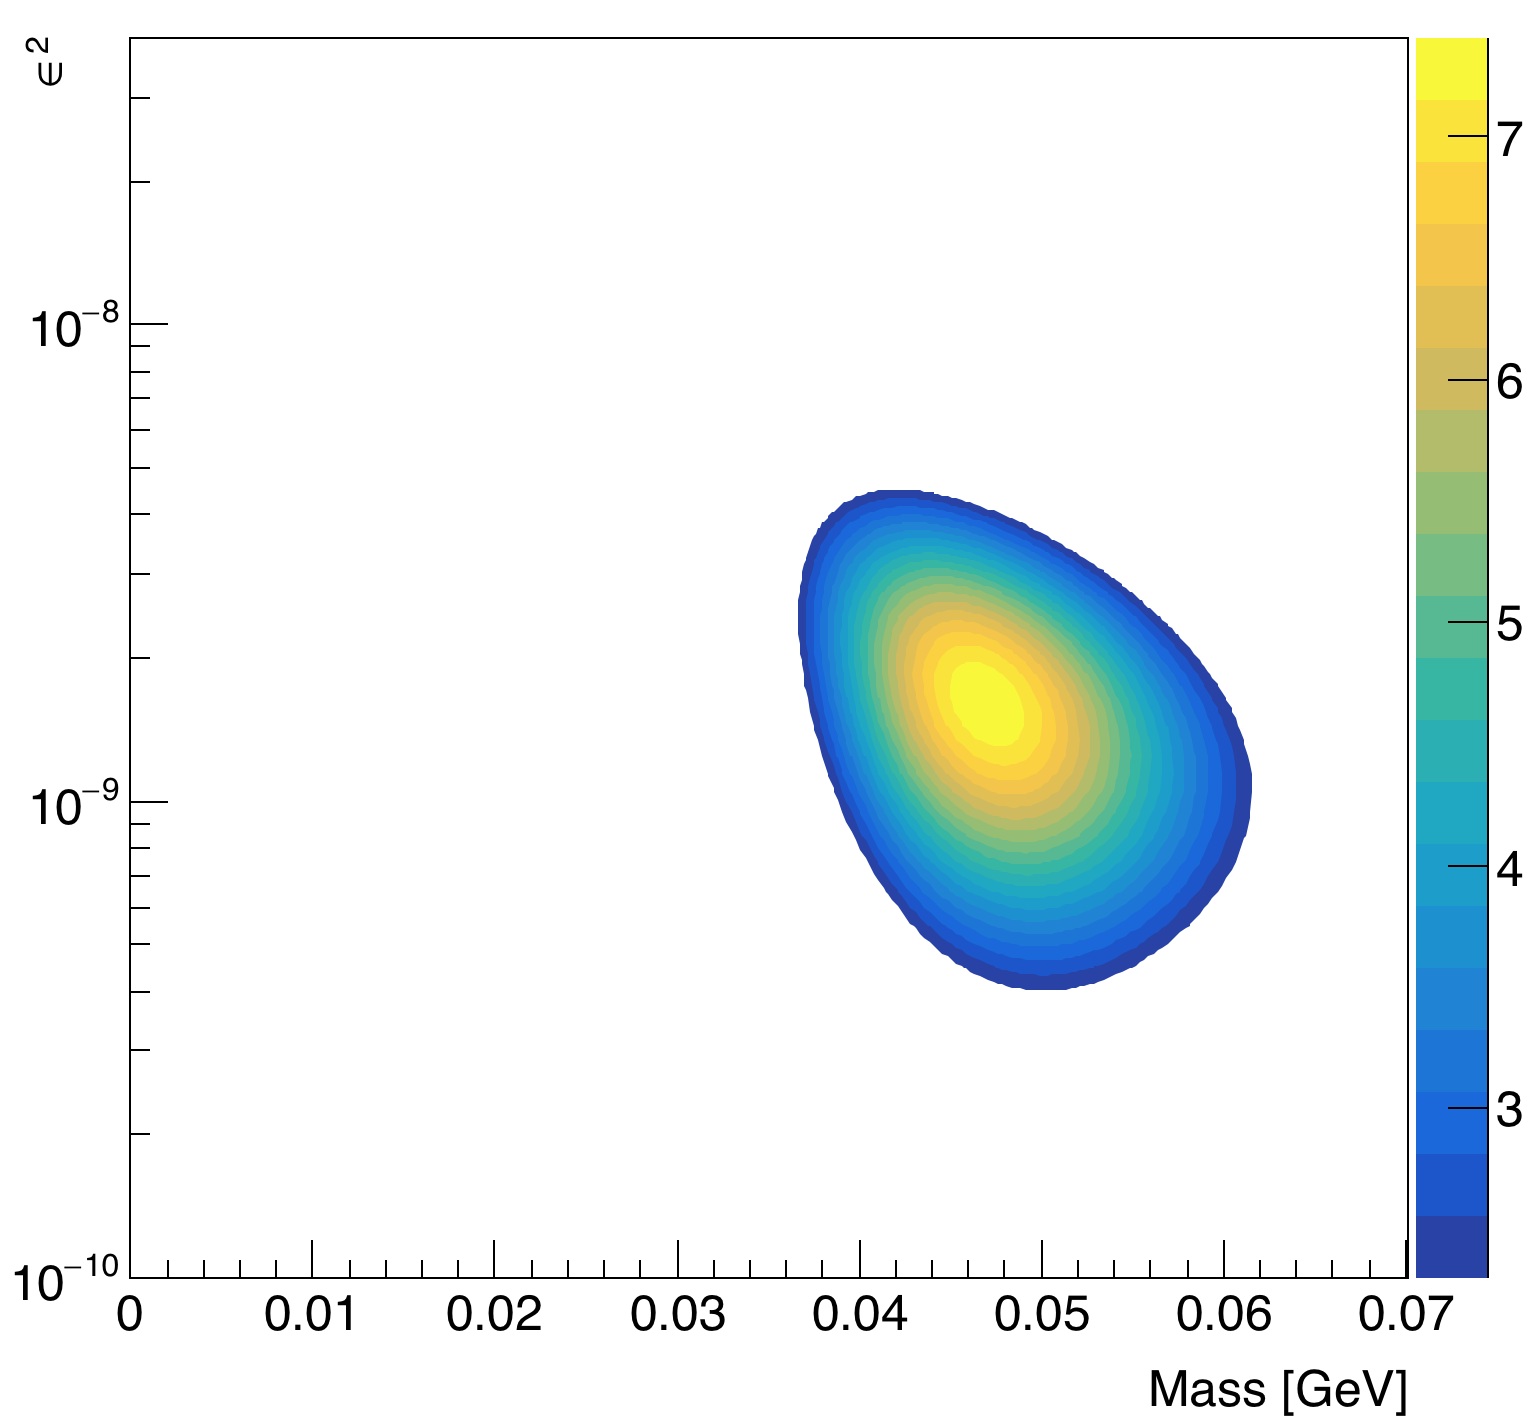
\includegraphics[width=0.55\textwidth]{pics/results/signal_1yr.png}
%  \caption[Projected reach for one year of running at 0.5~mm]{By projecting the measured $zCut$ from the L1L1 0.5~mm data and correspondingly increasing the statistics for one year of continuous running, the 90$\%$ CL reach is shown.}
%  \label{fig:reach_1yr}
%\end{figure} 
%
%While the signal yield is lower, it is interesting to note that for continuous running with the SVT at 1.5~mm, the first reach is attainable at 20~weeks of running. The 90$\%$ CL for 1~year of continuous running is somewhat similar to the the reach projected for the 0.5~mm running but peaks at a slightly higher mass. 
While the overall signal yield is lower (due to lower rates and less beam time), it is interesting to note that the background in the 1.5~mm data is much less than the background measured in the 0.5~mm data. The 1.5~mm data also has a slightly better vertex resolution across the mass range. If the rates can be handled by the detector and read out, then increasing the beam luminosity and running with the SVT at a slightly more open position may eliminate the excess high $z$ background. A comparison of the $z$ vertex resolution is shown in Figure~\ref{fig:vtxRes}. 

\begin{figure}[htb]
  \centering
      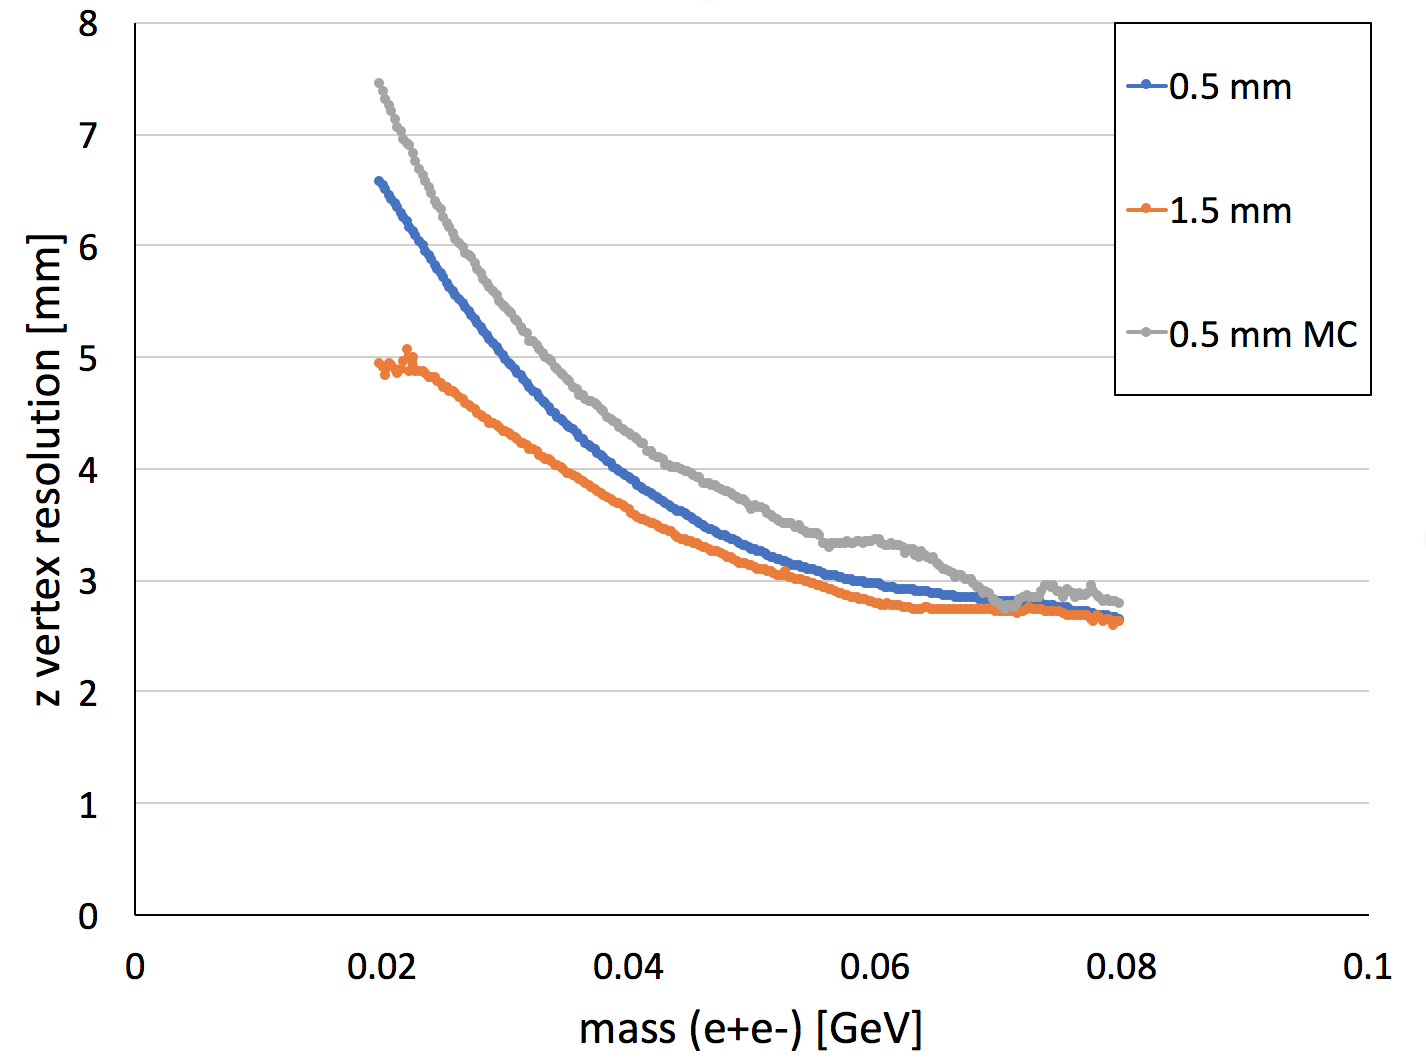
\includegraphics[width=0.75\textwidth]{pics/results/vtxRes.png}
  \caption[Vertex resolutions as measured in data and compared]{The $z$ vertex resolution is shown here as a function of mass where the resolution is obtained from the Gaussian fit to the core of the distribution. The resolution anticipated from MC is slightly worse than what was obtained from the data. The 1.5~mm data has a slightly better vertex resolution than the 0.5~mm data.}
  \label{fig:vtxRes}
\end{figure}

The reach projected from the proposal is very different from that derived from the experimental data. The primary difference is due to the proposal assumption that the reconstructed vertex efficiency was a constant 0.5 between the target and the first layer. This assumption neglected the geometric acceptance effects and the loss of smaller mass $A^{\prime}$s that decay far downstream of the target and miss the first SVT layer. This assumption is also why the peak in the mass of the proposal reach is much lower than in the data (25~MeV as opposed to 42~MeV). The second significant difference is that the beam exit hole in the ECal was not accounted for in the reach projections. From data and simulation, we know that we lose trident events when the electron goes through the electron hole, and the event is not triggered. Other differences between the proposal and the measured reach is the thickness of the target (proposed was 0.125$\%$ radiation thickness whereas the measured value was found to be 0.116$\%$), contamination due to excess backgrounds (such as wide angle bremsstrahlung), and time spent running. The wide angle bremsstrahlung triggered many events that were not anticipated and created some downstream $z$ vertex background contamination by interacting with the dead region of Layer 1. \\
\indent HPS is developing upgrades that will improve future running. We will add a charged particle hodoscope to the positron side of the ECal to veto triggers from photon clusters from wide angle bremsstrahlung and keep events where the electron is lost in the ECal electron hole. This should reduce some of the background and improve the trident yield. In addition, adding a Layer 0 SVT tracking plane at 5~cm downstream of the target should improve the vertex resolution by a factor of 2, which will enable tighter $zCut$s. This will extend the reach to include efficiency at smaller masses. The ability to set tighter $zCut$s does not eliminate the apparent high $z$ background events in the data. This source of excess background remains to be understood.

\subsection{Sources of systematic uncertainty}
Key sources of uncertainty in the vertex analysis arise from factors affecting the $zCut$ and the overall estimate of the number of $A^{\prime}$ produced for a given mass bin. Sources of uncertainty that affect the $zCut$ are primarily attributed to the mass resolution and the fit model used to extrapolate the $zCut$. The expected number of $A^{\prime}$ produced for a given mass bin is strongly determined by the radiative fraction from Monte Carlo. The reconstructed mass of the $e^+e^-$ pair is essential to both the $zCut$ calculation and the estimated statistics in each mass bin.\\
\indent The mass resolution is  a source for systematic uncertainty. The only comparison of the Monte Carlo with data comes from the M\o ller mass. The 17$\%$ difference between data and Monte Carlo was assumed to be a mass-independent systematic offset. If the scaled mass resolution from Equation~\eqref{eq:massresScaled} is incorrect, then the $zCut$ would change, affecting the overall anticipated signal counts and reach. Figure~\ref{fig:mResdub} shows the effect of doubling the mass resolution on the $zCut$ for the L1L1 0.5~mm data. 
\begin{figure}[htb]
  \centering
      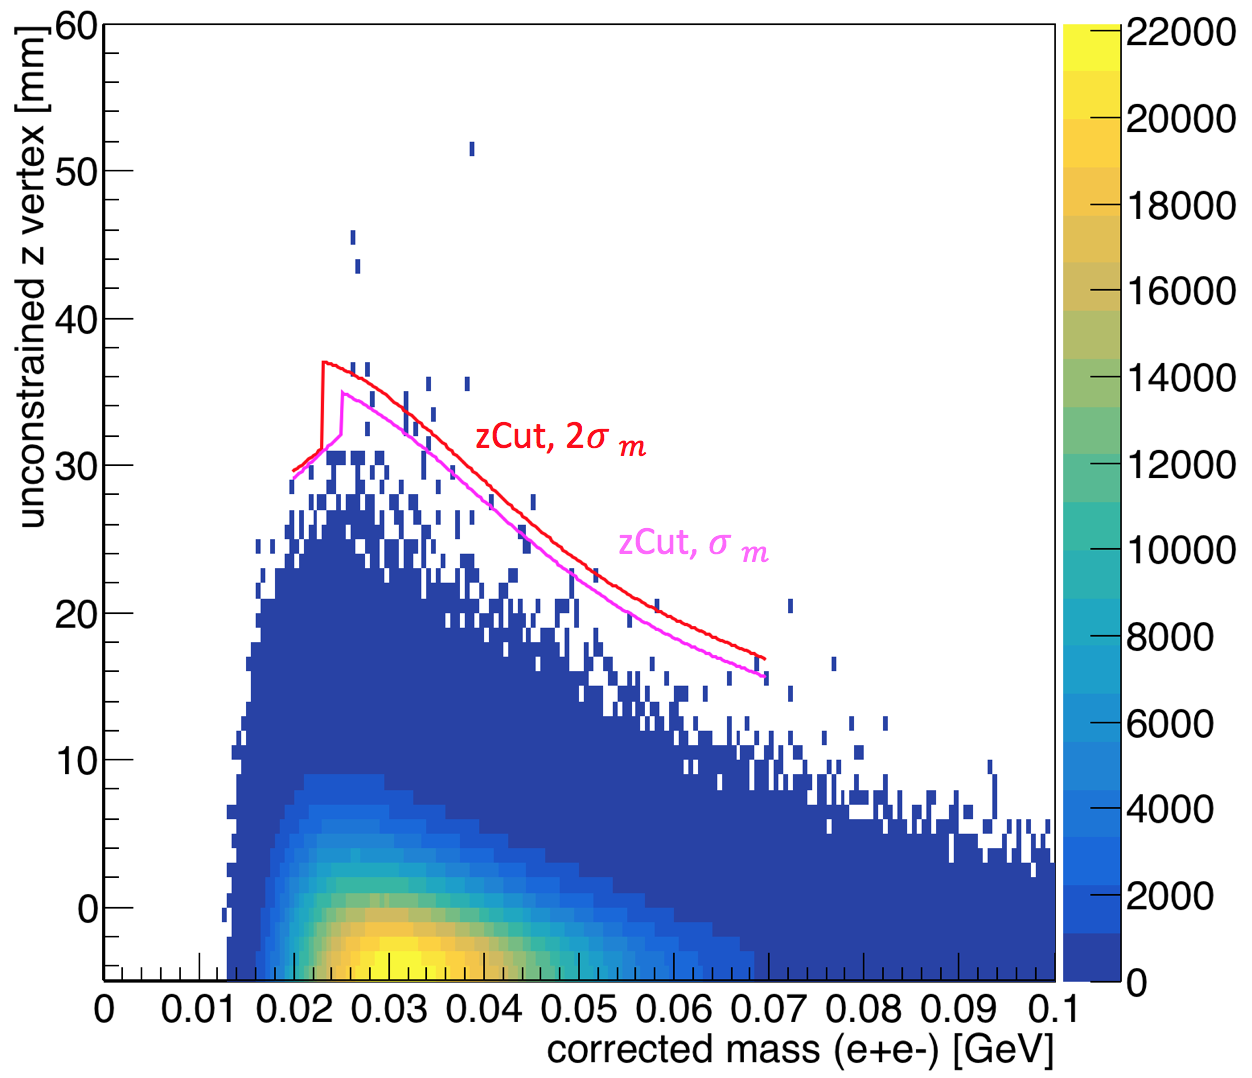
\includegraphics[width=0.75\textwidth]{pics/results/mres_systematics.png}
  \caption[$zCut$ when mass resolution is doubled]{The $zCut$ is recalculated (shown in red) assuming that the mass resolution is a factor of 2 worse than anticipated from Equation~\eqref{eq:massresScaled}. The $zCut$ using the mass resolution from Equation~\eqref{eq:massresScaled} is shown in magenta. The systematic difference between the two $zCut$s is approximately 1.5~mm. The total number of high $z$ events is reduced by 75$\%$.}
   \label{fig:mResdub}
\end{figure}
This increases the $zCut$ by approximately 1.5~mm, varying across the mass range. This shift reduces the number of high $z$ background events by approximately 30$\%$ from 24 to 16 events. It also reduces the number of expected signal events, calculated from Equation~\eqref{eq:signal}, by 15$\%$. The maximum expected signal events using the $zCut$ from the doubled mass resolution is 0.092 (compared to 0.109 found previously). The actual mass resolution is certainly much less than $2\sigma_m$. The $zCut$ is crucial to our anticipated reach and high $z$ background rejection.\\
\indent The reconstructed mass is a possible source of systematic uncertainty because this affects the number of events beyond the $zCut$ that are measured in a given mass bin. While we validated the mass reconstruction using the M\o ller mass comparison between data and Monte Carlo, there is no way to validate the reconstructed mass for displaced vertices and reconstructed pairs at different masses. It is possible that the mass correction from Equation~\eqref{eq:massCorrection} introduces a systematic offset of the reconstructed masses in data. Any offset in the reconstructed mass could put events into the wrong mass bins with a $z$ vertex dependence. For the masses and vertices measured in the L1L1 data, the uncorrected mass in Monte Carlo is presumably worse (as having been incorrect by as much as 50$\%$). Any inaccuracies in the vertex fitter and extracted mass should be exactly replicated by the Monte Carlo. The mass correction appears to significantly improve the mass resolution. Any remaining effect from the correction to the mass may move the event by as much as one mass bin, but presumably not more. This would not significantly alter the number of high $z$ background events but may change the number of high $z$ events in a single mass bin by a few events. Even so, due to the general uniformity of events beyond the $zCut$, this would not significantly change the results found. In order for the reconstructed mass to strongly change the number of statistics in a given mass bin (driven by the number produced in the prompt vertex region), the M\o ller mass would need to have been systematically different by at least 15$\%$. In short, the systematic offset in the reconstructed displaced vertices is more likely and serious than the possibility of mis-reconstructing the mass from prompt events, and the effect would probably not change the high $z$ background events observed by more than one mass bin. \\
\indent Agreement between the data and Monte Carlo is essential for estimating the radiative fraction in the final event sample. Any difference from the radiative fraction found in this dissertation systematically changes the estimated signal count beyond $zCut$. The radative fraction is found to be 9.5$\%$, but if there is a mass-dependence or offset of the radiatives generated by Monte Carlo, then the resulting expected signal counts could be very different. From preliminary work on understanding effects from tracking inefficiencies and contamination by WAB events, the radiative fraction and its estimated uncertainty is $9.5\pm3\%$. 

\subsection{Recommended improvements to vertex cuts}
For future HPS running, there are some optimized vertex cuts that could have been used for the vertex search here. These cuts were not fully realized until after unblinding, but should be noted for future analyses. While these cuts can reject some of the high $z$ background events, they also decrease the statistics of the distribution which changes the $zCut$. None of these cuts specifically removes all of the high $z$ background events. \\
\indent The cut on the track $\chi^2$ should really be a cut on the track $\chi^2$ per degree of freedom. The number of degrees of freedom in the track fit depends on the number of SVT layers hit, $n_{hits}$, as $2n_{hits}-5$. For L1L1 events with hits in both layers 1 and 2, a cut to the track $\chi^2$ per degree of freedom is not a significant change from a cut to the track $\chi^2$. For L1L2 events, this cut has more effect on the data because each event has at least one five-hit track. Preliminary analysis implementing this cut does not change the overall high $z$ driven $zCut$ of the L1L2 data, but could prove useful when further understanding the backgrounds from missing Layer 1 events. \\
\indent The track-cluster match $n\sigma$ parameter was kept loose for the vertex analysis as no immediate improvement was obtainable by tightening this cut. Based on the distribution of the track-cluster matching parameters from the final data sample, this cut should be changed from separate cuts on the electron and positron matching, to one cut on both the electron and positron matching such that $n\sigma_{e+}+n\sigma_{e-}<10$. This reduces the final number of events in each mass bin, but also removes events where only one track was well-matched at the ECal.\\
\indent  The beam spot constrained vertex fit quality is critical to the vertex analysis for removing events that do not have a momentum that projects well back to the beam spot position. This cut has been shown to crucially remove large backgrounds at high $z$. It may be possible to further improve the vertex analysis by correctly propagating the fit errors of the vertex to the displaced vertex (currently, this is not the case). By improving our estimation of the error to the vertex fit, both the unconstrained and beam spot constrained vertex fit information may be improved and may further remove excess high $z$ events. \\
\indent Some preliminary work was to done to cut on the correlations between the track kink parameters in layers 1--3 in the SVT. While this removed a few displaced high $z$ events, this does not remove all of them (as is still apparent after applying these cuts to the L1L2 data). It's possibly that further studies on the kinks and allowable track scattering may be able to improve track selection for the vertex search.